%%%%%%%%%%%%%%%%%%%%%%%%%%%%%%%%%%%%%%%%%%%%%%%%%%%
%% P3: Phenomenology of Particle Physics                         
%%
%% Author:  André Rubbia                   		 
%%
%% Figure 3.32 Illustration of high-energy particles being identified by consecutive types of subdetectors in a typical collider experiment.
%%
%% This work is licensed under the Creative Commons Attribution 4.0 International License. 
%% To view a copy of this license, visit http://creativecommons.org/licenses/by/4.0/ or 
%% send a letter to Creative Commons, PO Box 1866, Mountain View, CA 94042, USA.
%%
%%%%%%%%%%%%%%%%%%%%%%%%%%%%%%%%%%%%%%%%%%%%%%%%%%%

\documentclass[a4paper,10pt]{article}

\usepackage[T1]{fontenc}
\usepackage[utf8]{inputenc}
\usepackage{lmodern}
\usepackage[labelfont=bf]{caption}
\usepackage{upgreek}

\usepackage{tikz}
\usepackage{pgfplots}
\pgfplotsset{compat=1.17}
\usepgfplotslibrary{ternary}
\usepgfplotslibrary{fillbetween}
\usepgfplotslibrary{external}

\def\d{\mathrm{d}}

\begin{document}

%%%%%%%%%%%%%%%   FIGURE  %%%%%%%%%%%%%%%%%%%%%%%%%%%%%%
\begin{figure}[htb]
\begin{center}
\vspace{5mm}
    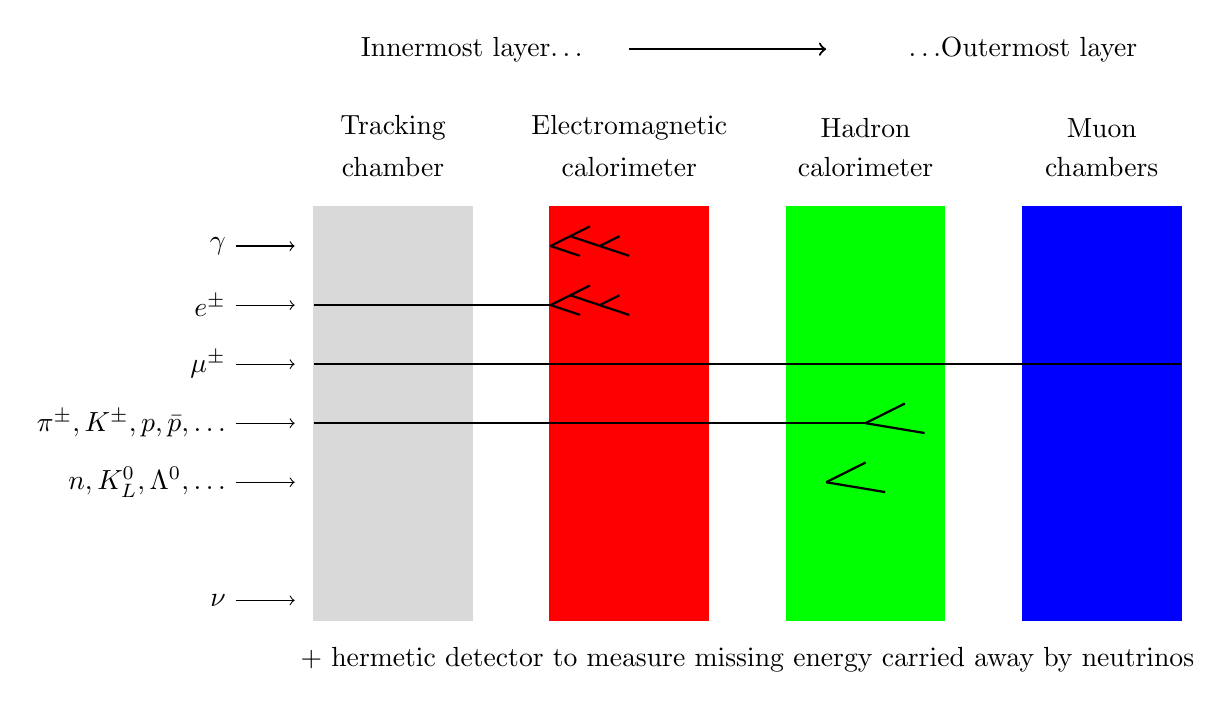
\begin{tikzpicture}[scale=0.5]
            \node at (4,12) {Innermost layer$\ldots$};
    	     \draw[thick,->] (8, 12)  -- +(5,0);
            \node at (18,12) {$\ldots$Outermost layer};

         \draw[thick,fill,color=black!15!white] (0,-2.5) rectangle +(4,10.5);
         \draw[thick,fill,color=red] (6,-2.5) rectangle +(4,10.5);
         \draw[thick,fill,color=green] (12,-2.5) rectangle +(4,10.5);
         \draw[thick,fill,color=blue] (18,-2.5) rectangle +(4,10.5);
%%         \draw[<-] (0.95,0.2) -- (1.,-0.1) node[below] {Beryllium target};
         \draw[->] (-2,7) node[left] {$\gamma$} -- (-0.5,7);
         \draw[thick] (6,7)  -- +(0.5,0.25);
         \draw[thick] (6,7)  -- +(0.75,-0.25);
         \draw[thick] (6.5,7.25)  -- +(0.5,0.25);
         \draw[thick] (6.5,7.25)  -- +(0.75,-0.25);
         \draw[thick] (7.25,7.)  -- +(0.5,0.25);
         \draw[thick] (7.25,7.)  -- +(0.75,-0.25);
         \draw[->] (-2,5.5) node[left] {$e^\pm$} -- (-0.5,5.5);
          \draw[thick] (0,5.5)  -- (6,5.5);
        \draw[thick] (6,5.5)  -- +(0.5,0.25);
         \draw[thick] (6,5.5)  -- +(0.75,-0.25);
         \draw[thick] (6.5,5.75)  -- +(0.5,0.25);
         \draw[thick] (6.5,5.75)  -- +(0.75,-0.25);
         \draw[thick] (7.25,5.5)  -- +(0.5,0.25);
         \draw[thick] (7.25,5.5)  -- +(0.75,-0.25);
         \draw[->] (-2,4) node[left] {$\mu^\pm$} -- (-0.5,4);
         \draw[thick] (0,4)  -- (22,4);
         \draw[->] (-2,2.5) node[left] {$\pi^\pm, K^\pm, p,\bar p, \ldots$} -- (-0.5,2.5);
         \draw[thick] (0,2.5)  -- (14,2.5);
          \draw[thick] (14,2.5)  -- +(1,0.5);
         \draw[thick] (14,2.5)  -- +(1.5,-0.25);
        \draw[->] (-2,1) node[left] {$n, K^0_L,\Lambda^0, \ldots$} -- (-0.5,1);
         \draw[thick] (13,1)  -- +(1,0.5);
         \draw[thick] (13,1)  -- +(1.5,-0.25);
         \draw[->] (-2,-2) node[left] {$\nu$} -- (-0.5,-2);
        \node at (11,-3.5) {+ hermetic detector to measure missing energy carried away by neutrinos};
%        \node at (4,4) {$\rho, A, Z, X_0, \lambda_I,\ldots$};
        \node at (2,10) {Tracking};
        \node at (2,9) {chamber};
        \node at (8,10) {Electromagnetic};
        \node at (8,9) {calorimeter};
        \node at (14,10) {Hadron};
        \node at (14,9) {calorimeter};
        \node at (20,10) {Muon};
        \node at (20,9) {chambers};
%        \node at (-11,5) {\emph{charged particles}};
%        \node at (-11,1.25) {\emph{neutral particles}};
     \end{tikzpicture}
\caption{Illustration of high-energy particles being identified by consecutive types of subdetectors
in a typical collider experiment. The curvature of the tracks in the magnetic field is not shown for
simplicity.}
\end{center}
\end{figure}
%%%%%%%%%%%%%%%   END FIGURE  %%%%%%%%%%%%%%%%%%%%%%%%%%%%%%
%

\end{document}
